\documentclass[french, 10pt]{beamer}

\usepackage[utf8]{inputenc}
\usepackage[T1]{fontenc}
\usepackage{lmodern}
\usepackage[french]{babel}
\usepackage{graphicx}

\usepackage{pgf}

\usepackage{tikz}
\usetikzlibrary{arrows,shapes}

\usetheme{Rochester}

%\usefonttheme{professionalfonts}
\definecolor{grenat}{RGB}{138,29,32}

\definecolor{neutral}{HTML}{E5E5E5}

\definecolor{alt1strong}{HTML}{2EA1DF}
\definecolor{alt1light}{HTML}{DFC3CA}
\definecolor{alt2strong}{HTML}{D79C35}
\definecolor{alt2light}{HTML}{DAC3DF}
\definecolor{alt3strong}{HTML}{2EDF98}
\definecolor{alt3light}{HTML}{DCDFC3}




\setbeamercolor{block title}{bg=grenat}
\setbeamercolor{block title example}{bg=alt2strong}
\setbeamercolor{block title alerted}{bg=grenat!60!red}

\setbeamercolor{block body}{bg=grenat!40}
\setbeamercolor{block body example}{bg=alt2strong!40}
\setbeamercolor{block body alerted}{bg=grenat!50!red!40}

\setbeamercolor{item}{fg=grenat}

\setbeamercolor{background canvas}{bg=grenat!10}

\setbeamercolor{title}{bg=grenat}
\setbeamercolor{frametitle}{bg=grenat}




\setbeamercovered{transparent}

\setbeamertemplate{navigation symbols}{}
\setbeamertemplate{footline}[text line]{\insertframenumber/\inserttotalframenumber}

%%%%\%%%%%%%%%%%%%%%%%%%%%%%%%%%%%%%%%%%%%%%%%%%
%% Introduction aux Systèmes d'exploitation  %%
%%   * Historique                            %%
%%   * Principes fondamentaux                %%
%%   * Grandes classes de systèmes           %%
%%%%%%%%%%%%%%%%%%%%%%%%%%%%%%%%%%%%%%%%%%%%%%%

\title{Systèmes d'exploitation, 2ème année}
\subtitle{Fichiers et processus}

\author{Yves \textsc{Stadler}}\institute{Université Paul Verlaine - Metz}

\date{\today}

\begin{document}


%%
% Page de Titre
%%
\begin{frame}
\titlepage
\end{frame}

\def\sectitle{Agenda}
\section{\sectitle}
\def\subsectitle{Plan du module}
\subsection{\subsectitle}

\begin{frame}{\sectitle}
\begin{block}{\subsectitle}
\begin{itemize}
\item Système de gestion des fichiers;
\item Gestion des processus (Parallélisme, threads, ordonnancement);
\item Synchronisation et concurrence;
\item Gestion de la mémoire;
\item Communications.
\end{itemize}
\end{block}
\end{frame}

\def\sectitle{Introduction}
\section{\sectitle}




\def\sectitle{Présentation générale d'un système d'exploitation}
\section{\sectitle}

\begin{frame}{\sectitle}

\def\subsectitle{Définition}
\subsection{\subsectitle}

\begin{exampleblock}{\subsectitle}
Extension logicielle du matériel dans le but d'offrir un service suffisant aux
utilisateurs.
\end{exampleblock}

\def\subsectitle{Objectif}
\subsection{\subsectitle}

\begin{block}{\subsectitle}
\begin{itemize}
    \item Masquer la complexité à l'utilisateur;
    \item Faciliter l'accès aux ressources.
\end{itemize}
\end{block}

\def\subsectitle{Types de systèmes d'exploitations}
\subsection{\subsectitle}

\begin{block}{\subsectitle}
\begin{itemize}
    \item mode d'exploitation différé;
    \item mode interactif d'exploitation, temps partagé;
    \item mode temps réel, système embarqués;
    \item mono-tâche, multi-tâches.
\end{itemize}
\end{block}
\end{frame}

\def\subsectitle{Organisation d'un système d'exploitation}
\subsection{\subsectitle}


\begin{frame}{\sectitle}
\begin{block}{\subsectitle}
\begin{itemize}
    \item Chaque système est basé sur un noyau (\textit{kernel});
    \item La noyau comprend deux parties : indépendante du matériel, dépendante
    du matériel;
\end{itemize}
\end{block}

\def\subsectitle{Partie dépendante}
\subsection{\subsectitle}
\begin{block}{\subsectitle}
\begin{itemize}
    \item gestion des interruptions;
    \item gestion mémoire;
    \item gestion des entrées sorties (E/S; IO).
\end{itemize}

\end{block}
\end{frame}

\def\subsectitle{Partie indépendante}
\subsection{\subsectitle}

\begin{frame}{\sectitle}
\begin{block}{\subsectitle}
\begin{itemize}
    \item ordonnanceur-distributeur;
    \item gestion des processus;
    \item paginiation, va-et-vient;
    \item sous-système de fichier;
    \item gestion des entrées sorties (partie "haute").
\end{itemize}
\end{block}


\end{frame}

\begin{frame}{\sectitle}

\def\subsectitle{Architecture UNIX}
\subsection{\subsectitle}

\begin{block}{\subsectitle}
\begin{itemize}
    \item Portabilité;
    \item Langage C;
    \item Processus arborescents.
\end{itemize}
\end{block}

\def\subsectitle{Unix}
\subsection{\subsectitle}

\begin{block}{\subsectitle}
\begin{itemize}
\item mono-tâche ou multi-tâches
\item temps partagé
\end{itemize}
\end{block}

\end{frame}


\def\sectitle{Présentation du noyau}
\section{\sectitle}
\def\subsectitle{Modèle en couche}
\subsection{\subsectitle}

\begin{frame}{\sectitle}
\begin{block}{\subsectitle}
Le système peut se présenter comme un ensemble de couches.
\end{block}

\begin{center}
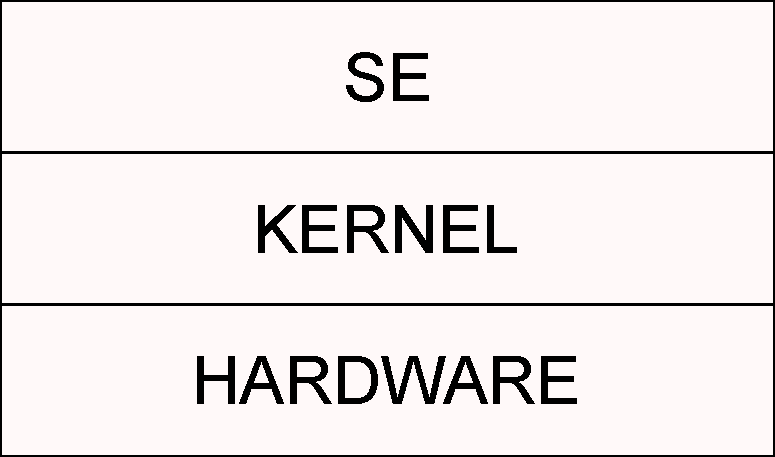
\includegraphics[width=0.75\textwidth]{images/Couches.pdf}
\end{center}

\end{frame}




\begin{frame}{\sectitle}

\begin{columns}[b]

\column{0.5\textwidth}
\begin{block}{\subsectitle}
\begin{itemize}
\item Le noyau ou kernel constitue une interface entre le matériel est les programmes
\item Il est lui même divisés en couches 
\item Il est irremplaçable par l'utilisateur
\item Il gère les processus, les périphériques, la mémoire
\end{itemize}
\end{block}

\column{0.5\textwidth}
\begin{center}
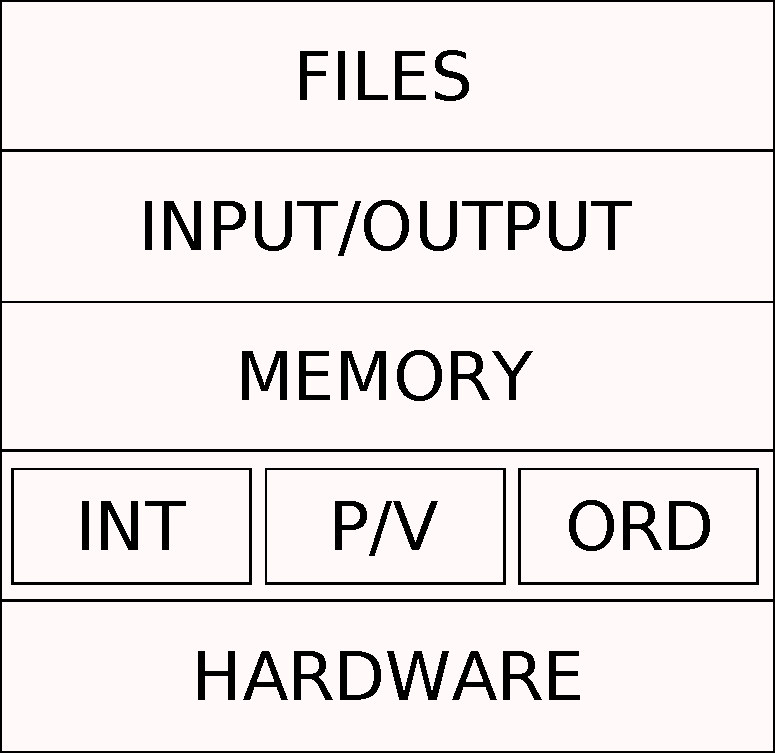
\includegraphics[width=\textwidth]{images/NoyauCouches.pdf}
\end{center}

\end{columns}
\end{frame}



\begin{frame}{\sectitle}

\def\subsectitle{Allocation de ressources}
\subsection{\subsectitle}

\begin{alertblock}{\subsectitle}
\begin{itemize}
    \item Rôle central du \textit{kernel} dans l'exécution des travaux:
    \begin{itemize}
        \item représentation et gestion des processus;
        \item gestion des interruptions;
        \item gestion des entrées, sorties.
    \end{itemize}
\end{itemize}
\end{alertblock}

\begin{figure}
\begin{center}
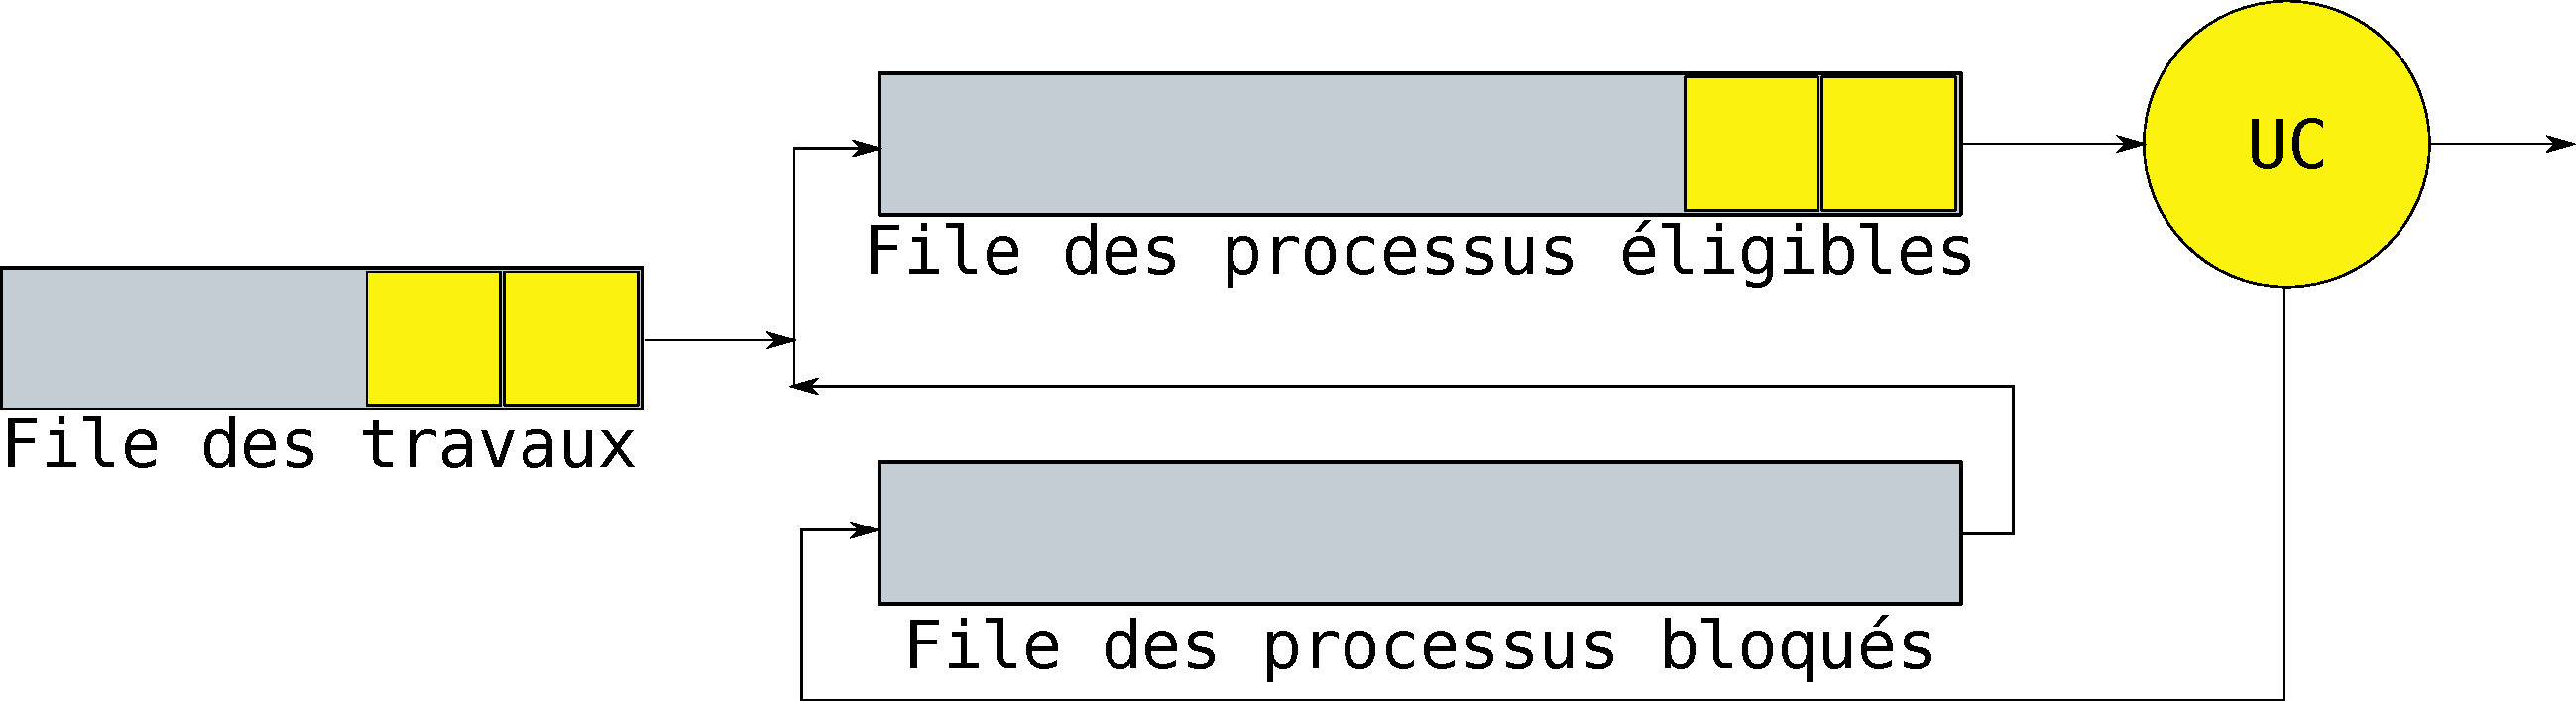
\includegraphics[width=\textwidth]{images/processFile.pdf}
\end{center}
\caption{Exemple de modèle d'allocation de l'UC}
\end{figure}

\end{frame}


\begin{frame}{\sectitle}
\def\subsectitle{Allocation de l'UC pour les systèmes mono-tâche}
\subsection{\subsectitle}
\begin{figure}
\begin{center}
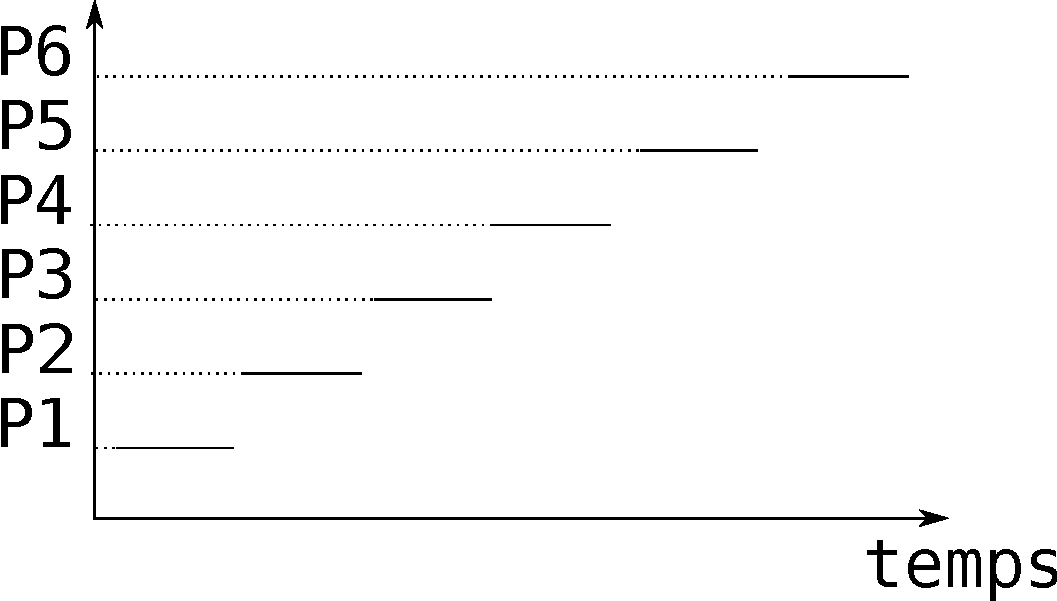
\includegraphics[width=\textwidth]{images/monoTache.pdf}
\end{center}
\caption{\subsectitle}
\end{figure}
\end{frame}

\begin{frame}{\sectitle}
\def\subsectitle{Allocation de l'UC pour les systèmes multi-tâches}
\subsection{\subsectitle}
\begin{figure}
\begin{center}
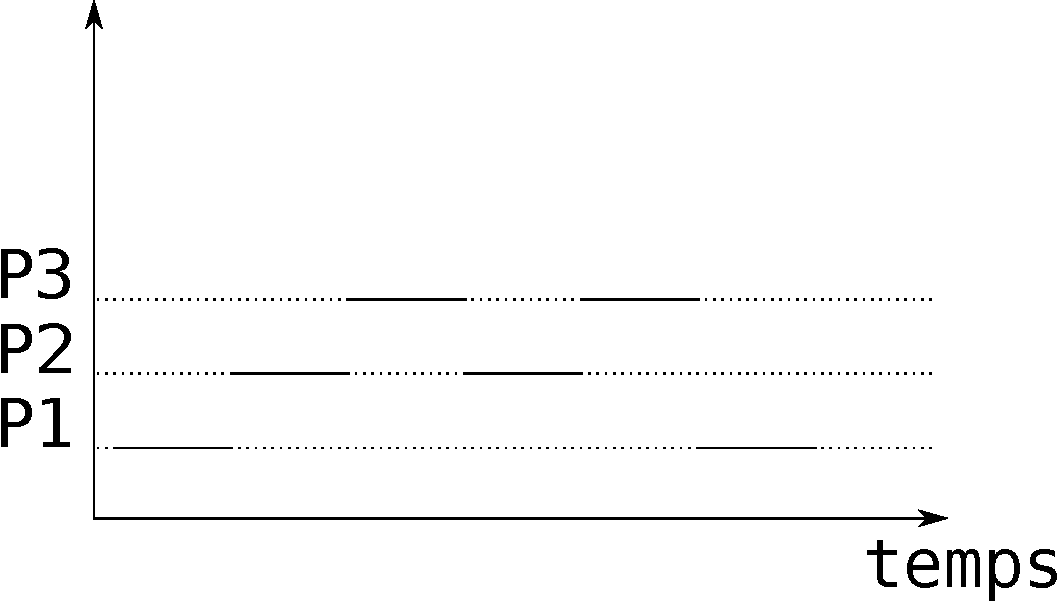
\includegraphics[width=\textwidth]{images/multiTaches.pdf}
\end{center}
\caption{\subsectitle}
\end{figure}

\end{frame}

\def\sectitle{Mécanisme de contrôle}
\section{\sectitle}
\begin{frame}{\sectitle}

\def\subsectitle{Mécanismes}
\subsection{\subsectitle}

\begin{block}{\subsectitle}
\begin{itemize}
    \item Les interruptions;
    \item les appels systèmes;
    \item les signaux horloge;
    \item les primitives de synchronisation.
\end{itemize}
\end{block}


\def\subsectitle{Les interruptions}
\subsection{\subsectitle}

\begin{block}{\subsectitle}
\begin{itemize}
    \item Événement suffisamment important pour nécessiter une interruption du
    système.
    \item Rapide, immédiat.
    \item généré aléatoirement par un périphérique ou par l'UC;
    \item peut-être générée par le système en interne, on parle alors de
    détournement.
\end{itemize}
\end{block}
\end{frame}

\section{\sectitle}
\begin{frame}{\sectitle}
\def\subsectitle{Rôle des interruptions}
\subsection{\subsectitle}
\begin{block}{\subsectitle}
\begin{itemize}
    \item Imposer les changement d'état de l'UC;
    \item Commutation de contexte, générée par une cause extérieur à
    l'instruction en cours.
\end{itemize}
\end{block}

\begin{alertblock}{\subsectitle}
\begin{itemize}
    \item L'UC doit être en mode interruptible;
    \item L'interruption doit être prioritaire aux autres interruptions;
\end{itemize}
\end{alertblock}

\end{frame}

\begin{frame}{\sectitle}
\def\subsectitle{Appel au superviseur - Définition}
\subsection{\subsectitle}

\begin{exampleblock}{\subsectitle}
\begin{itemize}
    \item Instruction qui a pour effet de provoquer une commutation de contexte
    du processeur.
\end{itemize}
\end{exampleblock}

\def\subsectitle{Appel au superviseur - Rôle}
\subsection{\subsectitle}
\begin{block}{\subsectitle}
\begin{itemize}
    \item Permettre l'appel depuis un programme d'une procédure du système
    nécessitant des droits étendus.
    \item Masquage interruption, \dots
\end{itemize}
\end{block}
\end{frame}


\def\subsectitle{Signaux d'horloge}
\subsection{\subsectitle}

\begin{frame}{\sectitle}
\begin{block}{\subsectitle}
\begin{itemize}
    \item Composant physique du système;
    \item Essentiel car il rythme le système;
    \item Génère des interruptions horloges.
\end{itemize}
\end{block}


\begin{exampleblock}{\subsectitle}
\begin{itemize}
    \item Affectation du temps dans le mot horloge
    \item Pendant l'activation du processus, le mot horloge est décrémenté de 1
    à chaque signal;
    \item Quand le mot vaut 0, un signal d'interruption est généré et le
    superviseur prend un décision.
\end{itemize}
\end{exampleblock}

\end{frame}


\begin{frame}{\sectitle}
\def\subsectitle{Primitives de synchronisation}
\subsection{\subsectitle}

\begin{block}{\subsectitle}
\begin{itemize}
    \item Nécessaires à l'asynchronisme;
    \item Nécessaire à la protection mutuelle;
    \item Plus que de simples appels de procédures.
\end{itemize}
\end{block}

\def\subsectitle{Exemple de l'exclusion mutuelle}
\subsection{\subsectitle}

\begin{exampleblock}{\subsectitle}
\begin{itemize}
    \item Deux processus A et B veulent mettre à jour le compte en banque
    d'Alice
    \item $C_{Alice} = C_{Alice} + Montant_{a}$ et $C_{Alice} = C_{Alice} +
    Montant_{b}$
    \item Quel est le résultat final ?
\end{itemize}
\end{exampleblock}

\end{frame}

\end{document}


